\documentclass[a4paper]{scrreprt}
%\documentclass[a4paper]{report}

% Uncomment to optimize for double-sided printing.
% \KOMAoptions{twoside}

% Set binding correction manually, if known.
% \KOMAoptions{BCOR=2cm}

% Localization options
\usepackage[english]{babel}
\usepackage[T1]{fontenc}
\usepackage[utf8]{inputenc}

% Enhanced verbatim sections. We're mainly interested in
% \verbatiminput though.
\usepackage{verbatim}

% PDF-compatible landscape mode.
% Makes PDF viewers show the page rotated by 90°.
\usepackage{pdflscape}

% Advanced tables
\usepackage{tabu}
\usepackage{longtable}

% Fancy tablerules
\usepackage{booktabs}

% Graphics
\usepackage{graphicx}

% Current time
\usepackage[useregional=numeric]{datetime2}

% Float barriers.
% Automatically add a FloatBarrier to each \section
\usepackage[section]{placeins}

% Custom header and footer
\usepackage{fancyhdr}
\setlength{\headheight}{15.2pt}
\pagestyle{fancyplain}

\usepackage{geometry}
\usepackage{layout}

% Math tools
\usepackage{mathtools}
% Math symbols
\usepackage{amsmath,amsfonts,amssymb}

\fancyhf{}
% Chapter header on non-plain pages only.
\lhead{\fancyplain{} {\leftmark}}
% Footer must contain print date. Ugly, but IPA requirement.
\lfoot{\printdate}
% Print date left and page count right was the thing which looked the
% most balanced.
\rfoot{\thepage}
% 
% Source code & highlighting
\usepackage{listings}

% Convenience commands
\newcommand{\mailsubject}{2407 - Computernetze - Practical exercise 1}
\newcommand{\maillink}[1]{\href{mailto:#1?subject=\mailsubject}
                               {#1}}

% Should use this command wherever the print date is mentioned.
\newcommand{\printdate}{\today}

\subject{2407 - Computernetze}
\title{Practical exercise 1}

\author{Michael Senn \maillink{michael.senn@students.unibe.ch}}

\date{\printdate}

% Needs to be the last command in the preamble, for one reason or
% another. 
\usepackage{hyperref}


\begin{document}
\maketitle

% \tableofcontents

\chapter{Router configuration}

Within \texttt{config.md} you will find the full configuration used on the
various routers.

On each router, the interfaces were configured by assigning them the desired
address, as well as static routing for the three subnets having been defined
where necessary.

\section{Used configuration directives}

\begin{description}
  \item[\texttt{conf t}]
    Enter interactive router configuration.
  \item[\texttt{end}]
    Exit interactive router configuration.
  \item[\texttt{interface}]
    Enter configuration specific to interface
  \item[\texttt{ip address}]
    Assign IP and network to interface.
  \item[\texttt{no shutdown}]
    Enable interface>
  \item[\texttt{no switchport}]
    Change interface into L3 mode.
  \item[\texttt{ip route}]
    Add static route.
  \item[\texttt{show ip route}]
    Show configured static routes.
\end{description}

\chapter{Ping between VMs}

Below you will find screenshots of pings of VM1 to VM2 and VM3, as well as of
VM2 to VM3.
\\
\\
\noindent\makebox[\textwidth]{
  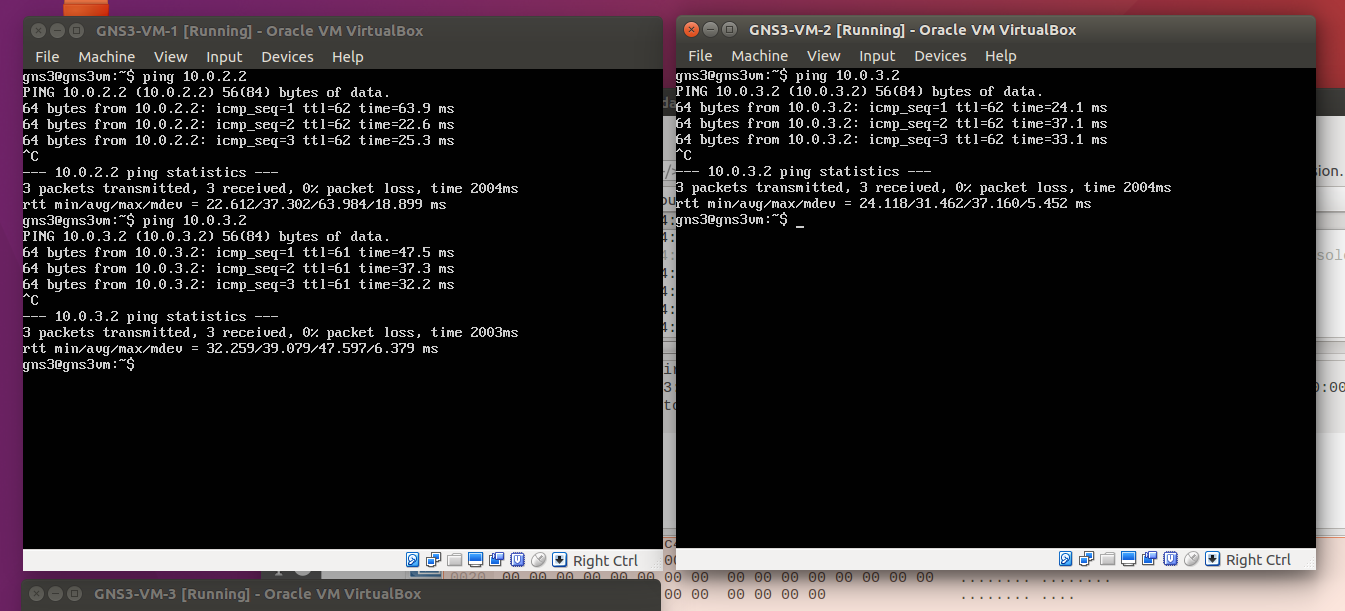
\includegraphics[width=\textwidth]{resources/ping_results.png}
}

\chapter{Network configuration of VMs}

Below you will find screenshots of the network configuration of all three VMs3.

All had DHCP disabled, and were statically configured to be in their respective
subnet, with the required IP address.
\\
\\
\noindent\makebox[\textwidth]{
  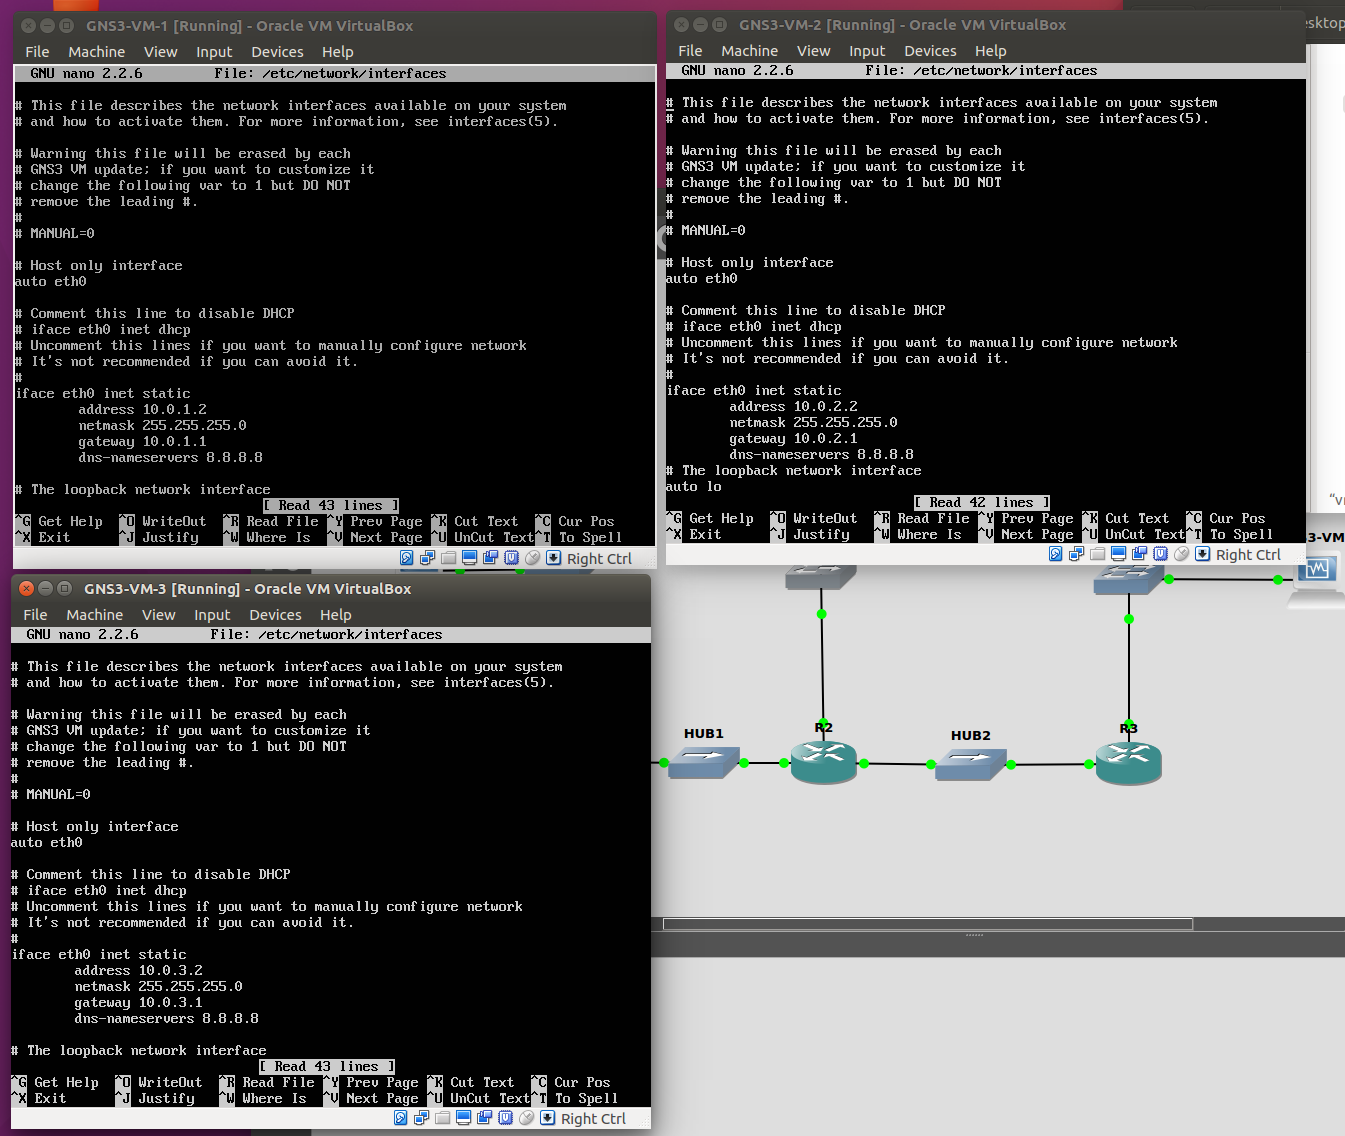
\includegraphics[width=\textwidth]{resources/network_configs.png}
}

\chapter{Wireshark capture of Hub 2}

Below you'll find a screenshot of the wireshark capture of one of the two ports
of hub 2. As hub 2 has 2 ports only, it should not matter of which one the
capture is.
\\
\\
\noindent\makebox[\textwidth]{
  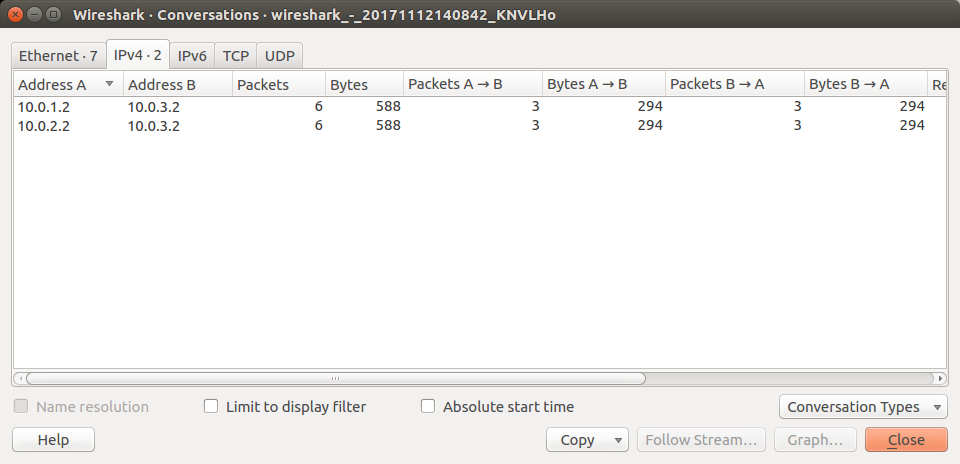
\includegraphics[width=\textwidth]{resources/wireshark_capture_statistics.png}
}

\end{document}

